\section{La maintenance: une tâche chronophage}
Dans un sondage réalisé par Agilent Technologies\footnote[1]{Agilent Technologies est une société 
qui développe et industrialise des instruments de mesure. Son siège se trouve à Santa Clara en 
Californie, https://www.agilent.com/}  demandait à des responsables de laboratoire de classer 
les tâches chronophages courantes qui ont le plus d’impact sur leurs analyses, nous pouvons 
constater les résultats suivants :
\begin{figure}[hp]
    \centering
    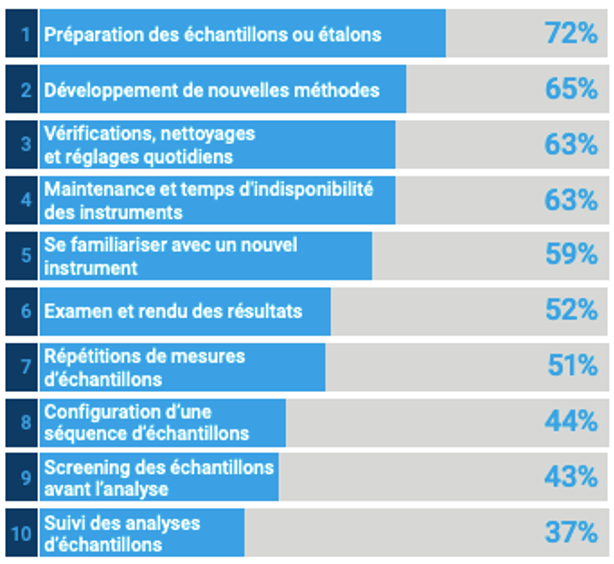
\includegraphics[scale=1]{images/sondage_chronophage.png}
    \caption{Résultats du sondage Agilent Technologies}
\end{figure}

On pense souvent à tort que les instruments sont complexes, chronophages et coûteux à entretenir.
Certains utilisateurs pensent également que leurs instruments analytiques continueront de 
fonctionner, jour après jour, sans aucun entretien ni attention. 
Quant aux laboratoires, ils sont nombreux à placer le temps d'indisponibilité des 
instruments parmi leurs plus grandes frustrations. Pourtant, les ingénieurs de maintenance 
constatent souvent qu’il suffit de nettoyer l’instrument ou d’effectuer un réglage de routine 
pour résoudre le problème. Ces tâches simples peuvent être effectuées par les analystes s’ils y 
sont formés. Avec des charges de travail élevées et une pression constante pour maximiser 
la productivité, les laboratoires commerciaux devraient mettre en place un calendrier de 
maintenance régulière pour garantir des performances instrumentales optimales et éviter 
les petits problèmes qui provoquent le temps d'indisponibilité des instruments pendant 
les analyses. Une bonne stratégie consiste à exécuter chaque jour un test de performances 
automatisé de l’instrument avant les analyses et à l’issue des analyses sans surveillance 
pendant la nuit. Les vérifications des performances permettent de confirmer l’état de l’instrument 
avant de démarrer les analyses. Cette vérification réduit les risques de devoir arrêter 
l’analyse et de remesurer les échantillons si les performances se dégradent pendant la journée.

De nombreux laboratoires incluent la maintenance et le nettoyage des instruments dans leur routine quotidienne ou leurs procédures opérationnelles normalisées. Mais le moment et la fréquence de ces activités peuvent être basés sur des défaillances d’instruments, d’anciens instruments ou des tâches effectuées pour différents types de solutions ou sur d’autres techniques d’analyse de métaux. À l’inverse, il est possible que les calendriers de nettoyage et de maintenance documentés dans les procédures de laboratoire soient omis ou négligés, notamment lorsque le laboratoire est soumis à des contraintes de temps. Ne pas exécuter ces tâches risque d’impacter les résultats, puisqu’il faudra résoudre le problème et éventuellement remesurer les échantillons, induisant une perte de temps.

Le sondage a montré que Près de 10\% des appels pour dépannage concernent un nettoyage de routine 
qui n’a pas été réalisé. Pour certains laboratoires, il est évident qu’une meilleure programmation 
de l’entretien courant peut éviter les pertes de temps liées à l’attente inutile d’un ingénieur de 
maintenance.

L’informatisation relative à la maintenance préventive aide les analystes à gérer leur calendrier 
de maintenance en leur permettant de configurer des alertes pour les tâches d’entretien courant. 
Cette dernière permet ainsi de paramétrer les fréquences de la maintenance et des vérifications 
quotidiennes pour qu’elles soient le mieux adaptées à la fréquence des maintenances requise pour 
tous types de solutions particuliers et à ne pas perdre de temps à réaliser une maintenance inutile.
L’autre grand avantage de l’informatisation de la maintenance est le fait qu’elle peut être utilisée comme preuve lors d’un audit. En fait, les laboratoires peuvent décider de mettre complètement de côté les calendriers de maintenance basés sur le temps et de supprimer les enregistrements de maintenance  sur papiers. 
La maintenance informatisée conserve toutes les données et s’occupe d’établir le calendrier de maintenance. Autre fonction utile : l’accès aux guides d’utilisation directement sur les moniteurs de maintenance. Un excellent moyen de gagner du temps et de s’assurer que les actions de maintenance sont effectuées correctement.
\pagebreak